\chapter{Grafisk teori}
\section{Grafisk brugergrænseflade} \label{chap:GUI}

I forbindelsen med udviklingen af systemet, skal man sørge for at designe det, så brugerne kan finde rundt i de forskellige funktioner. Da sejlklubben Sundets medlemmer kan bestå af en meget mangfoldig gruppe af mennesker, er det svært at indskrænke brugerne i en enkelt gruppe. Brugerne af systemet konkluderes derfor at kunne have meget forskellige evner inden for brugen af IT.

\subsection{Designet} \label{sec:Designet}

Programmets brugergrænseflade er designet ud fra principperne ifølge. \citep{gui1} 

\begin{itemize}
	\item Minimalisme
	\item Konsistente
\end{itemize}

Det betyder at der skal være så få forstyrrelser på skærmbilledet som muligt. Det skal være enkelt og simpelt at navigere rundt og finde de funktioner i programmet, man skal bruge. Der skal ikke være mange forskellige farver, og generelt skal programmet følge samme struktur til at navigere rundt igennem hele programmet. Herudover skal der ikke være en dyb menustruktur; helst ikke et dybere hierarki end 3.\fxnote{Er dette nu også korrekt?}

Disse forskellige principper eller retningslinjer, er forsøgt implementeret i systemet.

\subsection{Implementation}\label{sec:Implementation}

Menustrukturen består af tabs, som er store og lette at se. De forskellige funktioner i programmet er delt op i deres tilhørende tabs, og man kan altid gå ind i en ny tab uanset hvor, man befinder sig i programmet. Dette betyder, at strukturen ikke har et hierarki, da uanset hvor man befinder sig, kan der navigeres ind i alle programmets funktioner. Der er valgt blå nuancer, da det er en sejlklub, og dermed virkede som en logisk beslutning. Grunden til der ikke er flere farver rundt omkring i programmet, skyldes den minimalistiske, samt den konsistente, tankegang.

\fxnote{Her skal tilføjes nogle screenshots, så man kan se hvordan det helt konkret ser ud. Dette synes jeg dog skal vente til programmet når et mere færdigt stadie.}

Når brugergrænsefladen er lavet, skal den dermed også testes. Der vil blive forklaret hvordan dette vil blive gjort i et senere kapitel. \fxnote{Tilføj en kilde til kapitlet omhandlende test af programmets GUI}

\section{Windows Presentation Foundation}

\cbstart

Windows Presentation Foundation (WPF) er en grafisk brugergrænseflade på Windowsbaserede applikationer. 
WPF gør brug af  bl.a. vektorbaseret rendering af grafik, databinding, til nem redigering af data igennem den grafiske brugergrænseflade, og har også inkluderet Extensible Application Markup Language (XAML), hvilket er en nem måde at skabe WPF-grafik på.\citep{wpf} 

I dette projekt bruges WPF til at skabe den grafiske brugergrænseflade. Valget stod mellem WPF og Windows Forms (WinForms), hvilket er forgængeren til WPF til generering af grafik til Windows. 
Valget faldt på WPF, da XAML, som WinForms ikke har, gør det let at hurtigt lave en grafisk brugergrænseflade. 
Microsoft har også informeret om, at der ikke længere tilføjes nye funktioner til WinForms, men kun udelukkende rettelser af fejl.\citep{winforms}

En helt anden mulighed, som blev diskuteret, var at bruge en hjemmeside, som ville have den fordel, at den kan køre på stort set alle enheder, som har adgang til internettet via en browser. En hjemmeside, som gør brug af C\#, vil kunne laves lidt på samme måde som ved WPF; med HTML (HyperText Markup Language) og CSS (Cascading Style Sheets) som frontend og C\#-klasser som backend. 
En hjemmeside blev fravalgt, da det blev vurderet at WPF var nemmere at oprette end en hjemmeside, og at en grafisk brugergrænseflade ikke er en essentiel del af opgaven. 

\subsection{Ofte anvendte WPF-controls}
Det er ofte de samme WPF-controls, som anvendes til opbygningen af funktionaliteterne i den grafiske brugergrænseflade.
Disse vil blive beskrevet her.
På figur \ref{img:wpfdemo} vises de beskrevede elementer (Note: De 3 sidste elementer er henholdsvis DataGrid, ComboBox og ListBox).

\subsubsection*{ComboBox}
I WPF er en ComboBox det element, som andre steder omtales som en dropdown menu. 
Dens indhold kan instilles enten i XAML-koden eller i Code-Behind koden (her ment C\#-koden).
Hvis dette indhold skal være dynamisk, vil Code-Behind ofte være anvendt, eksempelvis hvis man kun vil have de medlemmer af en liste, som opfylder et givent prædikat. 

\subsubsection*{Button}
En Button er en knap, som kalder en metode i Code-Behind koden, når den trykkes. 
Den metode udfører det kode, som er angivet i den.

\subsubsection*{DataGrid}
Et DataGrid er et grafisk element, som kan vise data dynamisk.
Ofte vil det vise en liste af objekter.
Dets layout er opdelt i rækker og kolloner, hvor hver kollone indeholder en bestemt type data, og kan sorteres ved at klikke på labellet.
Det er også muligt at konstruere en søgefunktion, altså kan et DataGrid bliver filteret.

\begin{wrapfigure}[22]{R}{0.5\textwidth}
    \label{img:wpfdemo}
    \vspace{-30pt}
    \begin{center}
        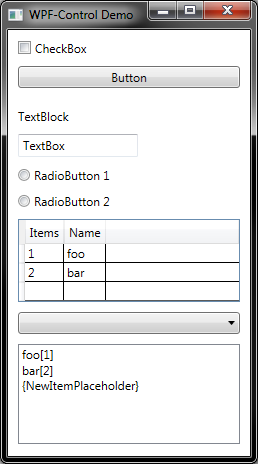
\includegraphics[width=0.48\textwidth]{UI/WPF-Demo.png}
    \end{center}
    \vspace{-15pt}
    \caption{Demonstration af WPFs Controls}
    \vspace{-15pt}
\end{wrapfigure}

\subsubsection*{CheckBox}
En CheckBox er en kvadratisk boks, som enten er ``Checked'' eller ikke ``Checked''. 
Dens stadie er binært, og (som standard) uafhængig af andre elementer.\fxnote{Måske give et eksempel på dette}

\subsubsection*{RadioButton}
En RadioButton er en cirkelformet CheckBox.
Dog vil RadioButtons ofte optræde i serie, altså 2 eller flere sammen.
Et oplagt brug af dem er til ja, nej (og måske) situationer, hvor kun er en af dem, man skal vælges.

\subsubsection*{StackPanel}
Et Stackpanel er ikke synligt for slutbrugeren, men bruges til at organisere de andre grafiske elementer.
Princippet er, at alle elementer i et StackPanel bliver skubbet sammen i mod en given retning.
Dette gør det nemmere at få de grafiske elementer til at flugte.
Derudover sikrer det en konsistent bredde af elementer deri, med mindre andet er angivet.

\subsubsection*{TextBlock}
En TextBlock bruges til afbildning af teksk, som ikke kan redigeres.
Det vil typisk være en forklarende tekst op ad et andet grafisk element.
Det er også muligt at ændre en TextBlock via Code-Behind. 
Hvis man vil føre en dialog med brugeren, eksempelvis til fejlbeskeder.

\subsubsection*{TextBox}
En TextBox er et tekstfelt, hvori brugeren kan skrive infomation. 
Dette kan dermed ses som et inputfelt. 
Det er også muligt at sætte sådan et felt til at være skrivebeskyttet, samt ændre dets indhold.

\subsubsection*{ListBox}
En ListBox er et tabel, med en kolonne og flere rækker, hvori en bruger kan vælge en eller flere elementer.
ListBoxen er i stand til at indeholde samlinger af data på enhver form, oftest vil det være en streng, men et billede er også en mulighed.
Den vil i nogen tilfælde have samme brugsscenarie som en ComboBox eller et DataGrid. 
Forskellen fra en ComboBox er, at der kan være flere synlige elementer i en ListBox på samme tid, samt der ikke er nogen dropdown menu.
Et DataGrid kan indeholde flere infomationer på kolonner, mens en ListBox kun kan indeholde en infomation.

\subsubsection*{UserControls}
Det er mulig at konstruere sine egne grænsefladeelementer fra et eller flere af WPFs indbyggede eller 3. parts Controls.
Dette kaldes en UserControl, som indeholder både en grafisk del og en Code-Behind del.
Det brugerskabte element kan derefter genbruges flere steder i programmet.
Dette er et eksempel på genanvendelse, hvilket kan bidrage til højere programkvalitet og større konsistens gennem programmet. 

\cbend